\section{\label{sec:init-pair-distribution} Pair distribution function}
The $n$-particle distribution function is defined via $n$-particle densities as follows (for reference, see Section~2.6 in~\cite{hansen2013theory})
\begin{equation*}
	\label{def:g_n}
	g^{(n)}(x_1,\dotsc,x_n)=\frac{\rho^{(n)}(x_1,\dotsc,x_n)}{\prod_{i=1}^{n}\rho^{(1)}(x_i)}
\end{equation*}
where $n$-particle density defined in the grand canonical ensemble is
\begin{eqnarray*}
	\label{def:rho_n}
	\rho^{(n)}(x_1,\dotsc,x_n) = \frac{1}{\Xi}\sum_{N=n}^{\infty} \frac{z^N}{(N-n)!} \int\exp(-\beta W_{N_v}(\gamma)) {\rm d} x_{n+1} \dotsc {\rm d} x_N.
\end{eqnarray*}
In this work, our goal is to calculate the pair distribution function $g^{(2)}(x_1, x_2)$
\begin{equation*}
	g^{(2)}(x_1, x_2) = \frac{\rho^{(2)}(x_1, x_2)}{\rho^{(1)}(x_1) \rho^{(2)}(x_2)}.
\end{equation*}
Thus we first need to calculate the one- and two-particle densities.

Let us first calculate $\rho^{(1)}$. By definition
\begin{equation*}
	\rho^{(1)} (x_1) = \Xi^{-1} \sum_{N=1}^{\infty} \frac{z^N}{(N-n)!} \int \exp(-\beta W_{N_v}(x_1, \dotsc, x_N)) {\rm d} x_2 \dotsc {\rm d} x_N.
\end{equation*}
Applying the method described in~\cite{KKD2020}, we obtain the following result
\begin{equation*}
	\rho^{(1)} (x_1) = \frac{K_1(\bar{y}, p, \mu)}{v K_0(\bar{y},p,\mu)} = \frac{\bar{n}(p,\mu)}{v}
\end{equation*}
where $\bar{n}$ is the average value of the occupation number of a cell. Thus, for the considered cell model with Curie-Weiss interaction we obtained the result known for homogeneous systems: the single-particle density is equal to the average particle density. In the presented theory, the average values are calculated using the probability measure $Q_{p,\mu}(n)$
\begin{equation*}
	Q_{p,\mu}(n) = \frac{1}{K_0(\bar{y}, p, \mu) n!} v^n \exp\left[(\bar{y} + \mu)n - \frac{a p}{2}n^2 \right],
	\quad n \in \mathbb{N}_0.
\end{equation*}
Thus
\begin{equation*}
	\bar{n}(p, \mu) \equiv \langle n \rangle_{Q} = \sum_{n=0}^{\infty} n Q_{p, \mu}(n),
\end{equation*}
and 
\begin{equation}
	\rho^{(1)}(x_1) = \frac{\langle n \rangle_{Q}}{v}.
\end{equation}

Let us now calculate the two-particle density, defined as
\begin{equation*}
	\rho^{(2)} (x_1, x_2) = \Xi^{-1} \sum_{N=2}^{\infty} \frac{z^N}{(N-n)!} \int \exp(-\beta W_{N_v}(x_1, \dotsc, x_N)) {\rm d} x_3 \dotsc {\rm d} x_N.
\end{equation*}
To deal with this expression, we again will follow the methodology developed in~\cite{KKD2020}. However, it is important to note that the result for $\rho^{(2)}(x_1, x_2)$ will vary depending on whether $x_1$ and $x_2$ belong to the same cell or to different cells.

When $x_1$ and $x_2$ belong to different cells, the result for $\rho^{(2)}(x_1, x_2)$ is as follows
\begin{eqnarray}
	\rho^{(2)} (x_1, x_2) & = & \left[\frac{K_1(\bar{y}, p, \mu)}{v K_0(\bar{y}, p, \mu)}\right]^2 
	= \frac{\bar{n}(p, \mu)^2}{v^2}
	\nonumber \\
	& = & \frac{\langle n \rangle_{Q}^2}{v^2}.
\end{eqnarray}
From this expression the result for $g^{(2)}(x_1, x_2)$ follows immediately
\begin{equation}
	g^{(2)}(x_1, x_2) = 1, \quad \text{ if } x_1, x_2 \text{ belong to different cells}.
\end{equation}
\begin{equation*}
	g^{(2)}(x_1, x_2) = 1, \qquad \text{ if } \nexists \Delta_l (x_1, x_2 \in \Delta_l).
\end{equation*}
\begin{equation*}
	g^{(2)}(x_1, x_2) = 1, \quad \text{ if } \forall \Delta_l (x_1 \notin \Delta_l \lor x_2 \notin \Delta_l).
\end{equation*}

When $x_1$ and $x_2$ belong to the same cell, the result for $\rho^{(2)}(x_1, x_2)$ is as follows
\footnote{compare with Eq.~(2.6.4) from~\cite{hansen2013theory}}
\begin{equation}
	\rho^{(2)}(x_1, x_2) = \frac{1}{v^2} \sum_{n=0}^{\infty} n(n-1) Q_{p, \mu}(n) 
	= \frac{\langle n(n-1) \rangle_{Q}}{v^2}.
\end{equation}
and for $g^{(2)}(x_1, x_2)$ one gets
\begin{equation}
	g^{(2)}(x_1, x_2) = \frac{\langle n(n-1) \rangle_{Q}}{\langle n \rangle_{Q}^2}, \quad \text{if } x_1, x_2 \text{ belong to the same cell}.
\end{equation}
\begin{equation*}
	g^{(2)}(x_1, x_2) = \frac{\langle n(n-1) \rangle_{Q}}{\langle n \rangle_{Q}^2}, \quad \text{if } \exists \Delta_l (x_1, x_2 \in \Delta_l).
\end{equation*}
In what follows, we will mostly focus on $g^{(2)}(x_1, x_2)$ with $x_1$ and $x_2$ in the same cell.
First thing to note is that given $x_1$ and $x_2$ belong to the same cell, the $2$-particle density does not otherwise depend on the position of the particles, thus we can just write $\rho^{(2)}$ for simplicity. The same consequently applies to $g^{(2)}$.

Before proceeding with numerical and graphical results for the pair distribution function $g^{(2)}$ let us first rewrite it in a few alternative representations.

{\it I}\\
Note that
\begin{eqnarray*}
	\rho^{(2)} & = & \frac{1}{v^2 K_0(\bar{y}, p, \mu)} \sum_{n=2}^{\infty} n(n-1) \frac{v^n}{n!} \exp\left[(\bar{y} + \mu)n - \frac{a p}{2} n^2\right]
	\\
	& = & \frac{1}{v^2 K_0(\bar{y}, p, \mu)} \sum_{n=0}^{\infty} (n^2 - n) \frac{v^n}{n!} \exp\left[(\bar{y} + \mu)n - \frac{a p}{2} n^2\right]
	\\
	& = & \frac{K_2(\bar{y}, p, \mu) - K_1(\bar{y}, p, \mu)}{v^2 K_0(\bar{y}, p, \mu)}
\end{eqnarray*}
and for $g^{(2)}$ one obtains
\begin{eqnarray}
	g^{(2)} & = & \frac{\left[K_2(\bar{y}, p, \mu) - K_1(\bar{y}, p, \mu)\right] K_0(\bar{y}, p, \mu)}{K_1(\bar{y}, p, \mu)^2}
\end{eqnarray}

{\it II}\\
In~\cite{MpkDob2022} the following change of variables was performed
\begin{equation*}
	\bar{y} + \beta\mu = \bar{z}.
\end{equation*}
The convenience of such change of variables consists in possibility to present some equations in parametric form, with $z$ being the parameter. In particular, the chemical potential can be written as a function of two variables $(\bar{z}, p)$
\begin{equation*}
	\beta\mu = \bar{z} - p K_1(\bar{z},p)/K_0(\bar{z},p).
\end{equation*}
Now, the pair distribution function takes on the form
\begin{equation}
	g^{(2)} = \frac{\left[K_2(\bar{z}, p) - K_1(\bar{z}, p)\right] K_0(\bar{z}, p)}{K_1(\bar{z}, p)^2}.
\end{equation}

{\it III} \\
For the average value of $n$ note the following:
\begin{eqnarray*}
	K_0(\bar{z}, p) \langle n \rangle_Q & = & 
	v^{-1} \sum_{n=1}^{\infty} n \frac{v^n}{n!} \exp(\bar{z}n - \frac{ap}{2}n^2)
	\\
	& = & \sum_{n=1}^{\infty} \frac{v^{n-1}}{(n-1)!} \exp(\bar{z}n - \frac{ap}{2}n^2)
	\\
	& = & \left| n=m+1; \quad \sum_{n=1}^{\infty} \rightarrow \sum_{m=0}^{\infty}; \quad n^2 = m^2 + 2m + 1 \right|
	\\
	& = & \exp(\bar{z} - \frac{ap}{2}) \sum_{n=0}^{\infty} \frac{v^n}{n!} \exp\left[(\bar{z} - ap)n - \frac{ap}{2}n^2 \right]
	\\
	& = & \exp(\bar{z} - \frac{ap}{2}) \langle \exp(-apn) \rangle_Q
	\\
	& = & \exp(\bar{z} - \frac{ap}{2}) K_0 (\bar{z} - ap, p),
\end{eqnarray*}
and thus
\begin{equation*}
	\langle n \rangle_Q = \frac{K_0(\bar{z} - ap, p)}{K_0(\bar{z}, p)} \exp(\bar{z} - \frac{ap}{2})
\end{equation*}

For the average value of $n(n-1)$ note the following
\begin{eqnarray*}
	K_0(\bar{z}, p) \langle n(n-1) \rangle_Q & = & 
	v^{-2} \sum_{n=2}^{\infty} n(n-1) \frac{v^n}{n!} \exp(\bar{z}n - \frac{ap}{2}n^2)
	\\
	& = & \sum_{n=2}^{\infty} \frac{v^{n-2}}{(n-2)!} \exp(\bar{z}n - \frac{ap}{2}n^2)
	\\
	& = & \left| n=m+2; \quad \sum_{n=2}^{\infty} \rightarrow \sum_{m=0}^{\infty}; \quad n^2 = m^2 + 4m +4 \right|
	\\
	& = & \exp(2\bar{z} - 2ap) \sum_{n=0}^{\infty} \frac{v^n}{n!} \exp\left[(\bar{z} - 2ap)n - \frac{ap}{2}n^2 \right]
	\\
	& = & \exp(2\bar{z} - 2ap) \langle \exp(-2apn) \rangle_Q
	\\
	& = & \exp(2\bar{z} - 2ap) K_0(\bar{z} - 2ap, p),
\end{eqnarray*}
and thus
\begin{equation*}
	\langle n(n-1) \rangle_Q = \frac{K_0(\bar{z} - 2ap, p)}{K_0(\bar{z}, p)} \exp(2\bar{z} - 2ap).
\end{equation*}

The pair distribution function takes on the form
\begin{equation}
	g^{(2)} = \exp(-ap) \frac{K_0(\bar{z} - 2ap, p) K_0(\bar{z}, p)}{K_0(\bar{z}-ap, p)^2}
\end{equation}
Note that the factor $\exp(-ap)$ is the low-density limit of the pair distribution function that can be obtained from the Boltzman factor of the interaction potential, see Appendix~\ref{sec:low-dens}.

\begin{figure}[htbp]
	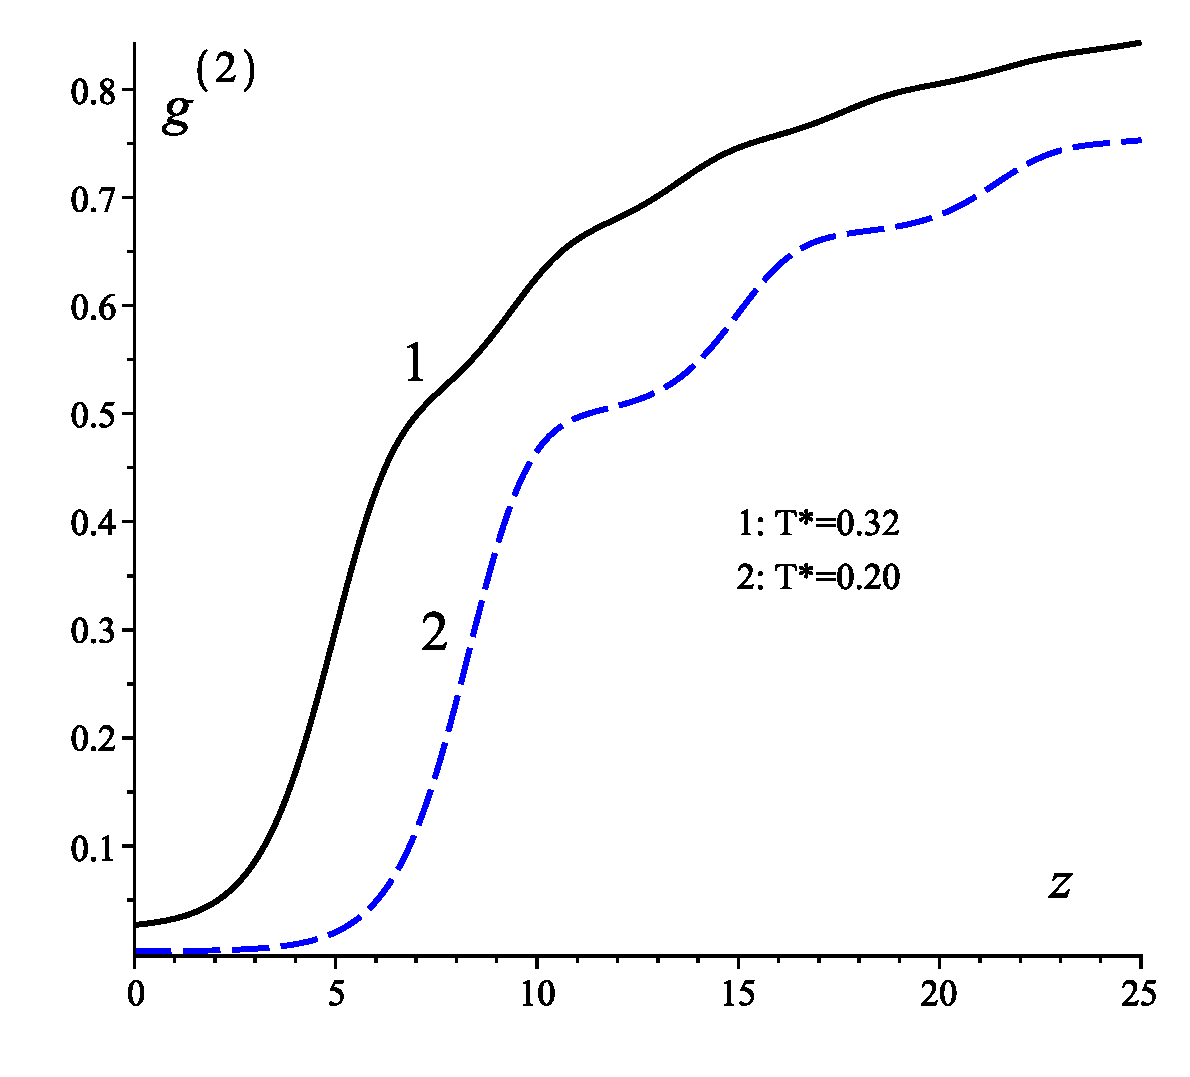
\includegraphics[width=0.7\textwidth,angle=0]{g2_vs_z}
	\caption{Pair distribution function $g^{(2)}$ versus $\bar{z}$.}
	\label{fig:g2_z}
\end{figure}
\begin{figure}[htbp]
	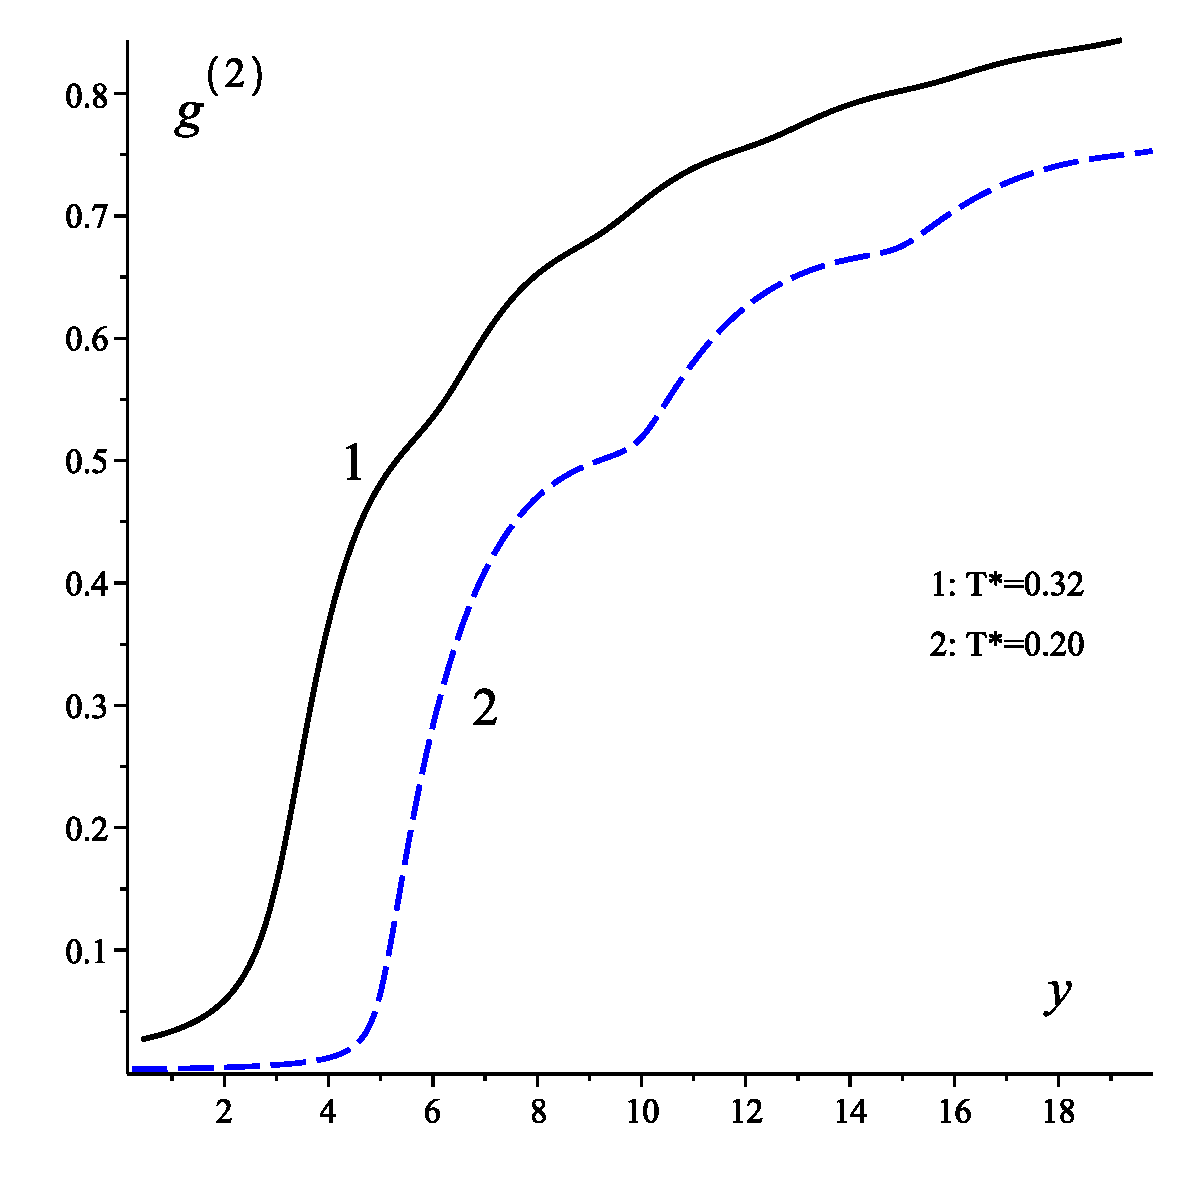
\includegraphics[width=0.7\textwidth,angle=0]{g2_vs_y}
	\caption{Pair distribution function $g^{(2)}$ versus $\bar{y}$.}
	\label{fig:g2_y}
\end{figure}

\begin{figure}[htbp]
	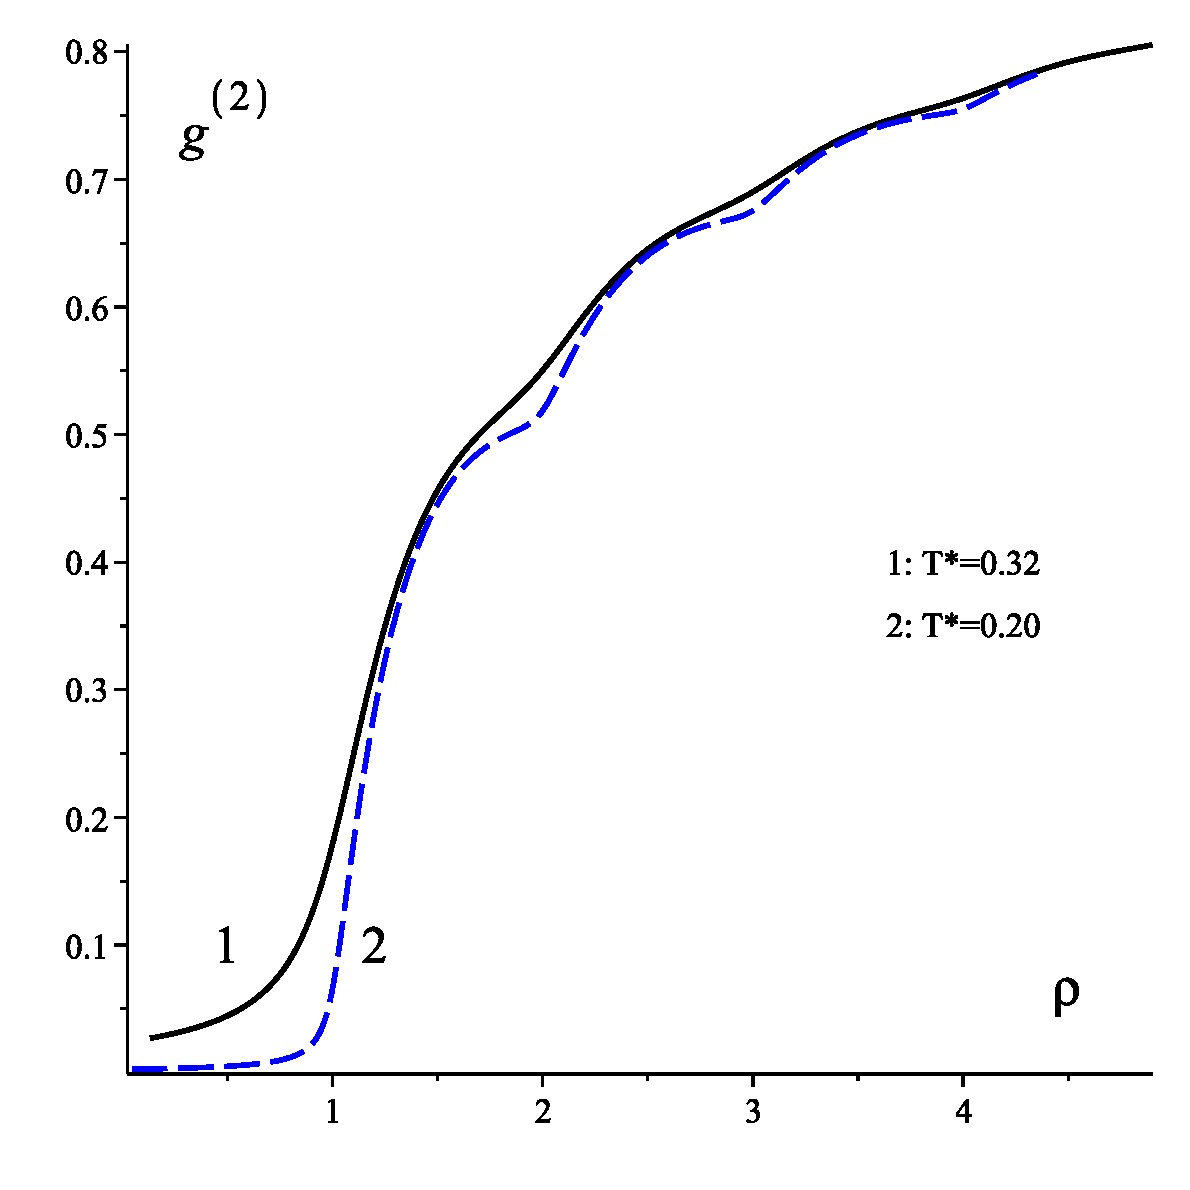
\includegraphics[width=0.7\textwidth,angle=0]{g2_vs_rho}
	\caption{Pair distribution function $g^{(2)}$ versus $\rho$.}
	\label{fig:g2_rho}
\end{figure}

\begin{figure}[htbp]
	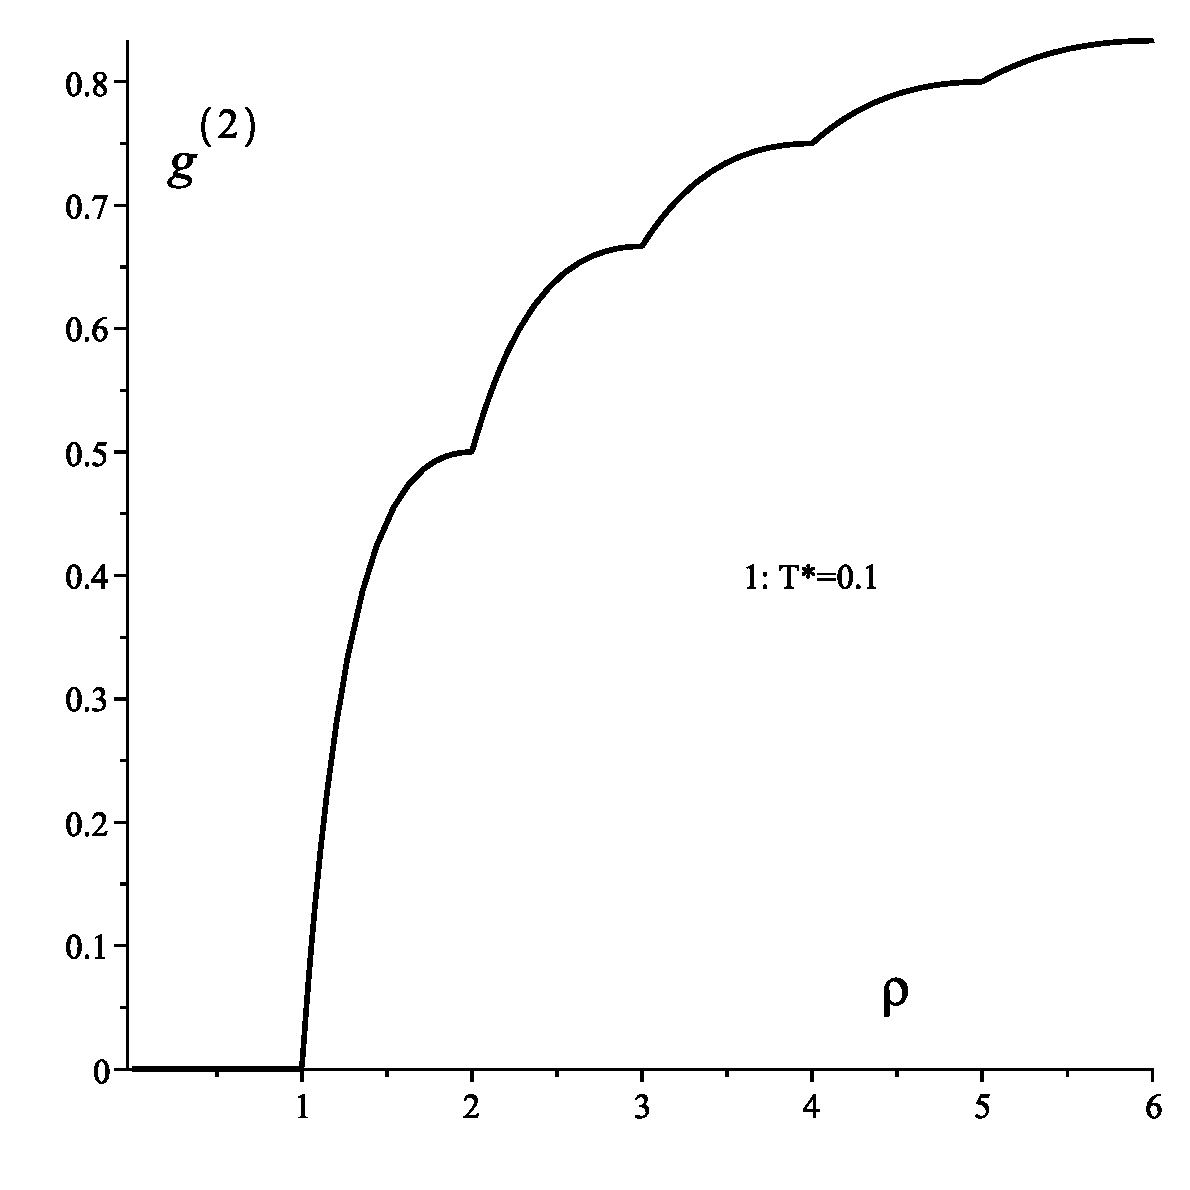
\includegraphics[width=0.7\textwidth,angle=0]{g2_vs_rho_low_temp}
	\caption{Pair distribution function $g^{(2)}$ versus $\rho$ at low temperature $T^*=0.1$.}
	\label{fig:g2_rho_low_temp}
\end{figure}

In Figure~\ref{fig:g2_z} the pair distribution function is shown as a function of $\bar{z}$ for two different values of temperature: $T^*=0.32$, which is above the range of critical temperatures, and $T^*=0.20$, which is below the range of critical temperatures. 

In Figure~\ref{fig:g2_y} the pair distribution function is shown as a function of $\bar{y}$ for the same temperatures.

In Figure~\ref{fig:g2_rho} the pair distribution function is shown as a function of density $\rho$ for the same temperatures.

Very interesting behavior of $g^{(2)}$ is observed in Figure~, where the dependency on density is presented in the low temperature limit, namely for $T^*=0.1$ 


